
\documentclass[a4paper,12pt]{article}

\usepackage[margin=1.5cm]{geometry}
\usepackage[T1]{fontenc}
\usepackage{lmodern}
\usepackage{tikz}
\usetikzlibrary{arrows.meta,calc}

\pagestyle{empty}

\begin{document}

\begin{center}
    {\Large\bfseries UML Class Diagram}\\[4pt]
    {\large Employee--LeaveBalance Composition}
\end{center}

\vspace{1cm}

\begin{center}
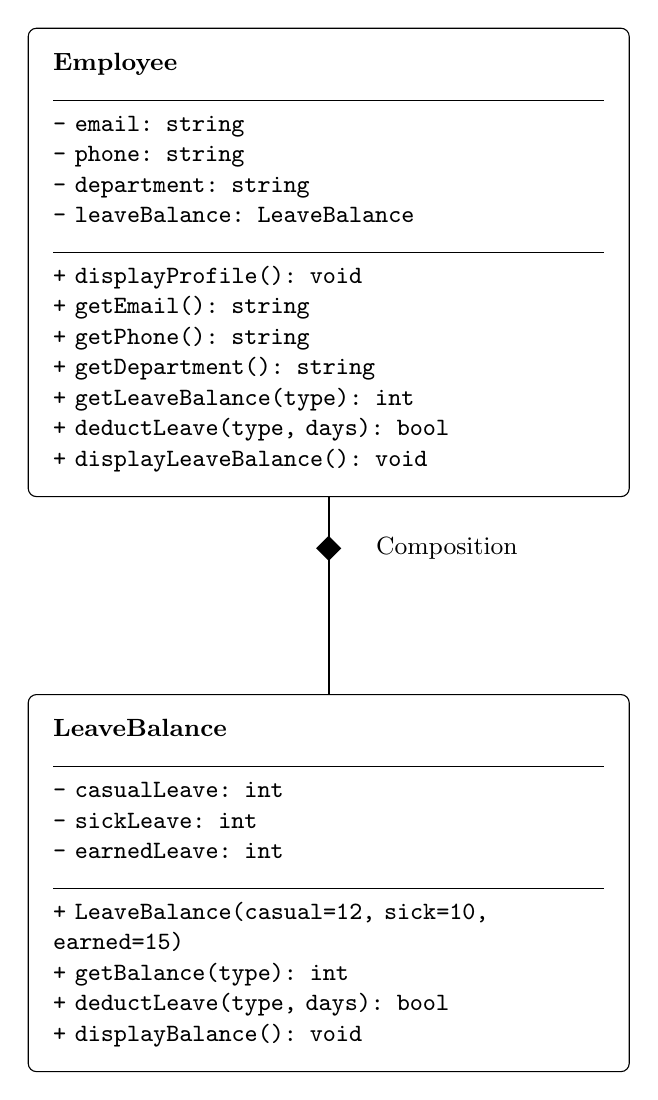
\begin{tikzpicture}[
    classbox/.style={
        draw,
        rounded corners=3pt,
        align=left,
        text width=7cm,
        inner sep=9pt,
        font=\small
    }
]

% Employee class
\node[classbox,anchor=north] (employee) at (0,0) {
    \textbf{Employee}\\
    \rule{\linewidth}{0.4pt}\\
    \texttt{- email: string}\\
    \texttt{- phone: string}\\
    \texttt{- department: string}\\
    \texttt{- leaveBalance: LeaveBalance}\\
    \rule{\linewidth}{0.4pt}\\
    \texttt{+ displayProfile(): void}\\
    \texttt{+ getEmail(): string}\\
    \texttt{+ getPhone(): string}\\
    \texttt{+ getDepartment(): string}\\
    \texttt{+ getLeaveBalance(type): int}\\
    \texttt{+ deductLeave(type, days): bool}\\
    \texttt{+ displayLeaveBalance(): void}
};

% LeaveBalance class, positioned relative to Employee
\node[classbox,anchor=north]
    (balance) at ($(employee.south)+(0,-2.5)$) {
    \textbf{LeaveBalance}\\
    \rule{\linewidth}{0.4pt}\\
    \texttt{- casualLeave: int}\\
    \texttt{- sickLeave: int}\\
    \texttt{- earnedLeave: int}\\
    \rule{\linewidth}{0.4pt}\\
    \texttt{+ LeaveBalance(casual=12, sick=10, earned=15)}\\
    \texttt{+ getBalance(type): int}\\
    \texttt{+ deductLeave(type, days): bool}\\
    \texttt{+ displayBalance(): void}
};

% Composition relationship
% Filled diamond at the Employee end
\coordinate (diamond) at ($(employee.south)+(0,-0.65)$);

\draw[thick] (employee.south) -- (diamond);

\fill
    ($(diamond)+(0,0.16)$) --
    ($(diamond)+(-0.16,0)$) --
    ($(diamond)+(0,-0.16)$) --
    ($(diamond)+(0.16,0)$) -- cycle;

\draw[thick] (diamond) -- (balance.north);

\node[font=\small,fill=white,inner sep=3pt]
    at ($(diamond)+(1.5,0)$) {Composition};

\end{tikzpicture}
\end{center}

\vspace{0.8cm}

\noindent\textbf{Relationship:} The \texttt{Employee} class contains a
\texttt{LeaveBalance} object as a member. This is represented as
composition in the UML diagram.

\end{document}
